\chapter{Ludmila Zahradnik}

The sun was beginning to cross into the west when the last of the supplies were organized and sent on their way. As the completion of her task drew closer, she thought she could feel the tension of the village rise in the air. It was equal parts excitement and uncertainty; resolve and trepidation. Though most of the adults in the village undertook patrols in the surrounding woodlands regularly, not many of those present had actually travelled beyond the borders of the barony itself.

 

With all her assistants having returned home to tend to their own families, Ludmila was once again left to the emptiness of the family manor. Closing the village ledger, she rose from her desk, looking to the wall near the door. Lined up neatly against it was a row of baggage lightly packed for the journey: her family’s clothing and personal effects sorted away in the spare moments of time that she had to herself. Despite her dearly held hopes, however, no sail had appeared on the river, nor did anyone else arrive over land. With the priority now to escape the Kingdom as quickly as was reasonable, there was no longer time left to wait. She placed the ledger in her pack before making one last round of the makeshift manor, but with as little personal activity as it had seen, there was not much to tidy or secure. She drew the thick curtains over the windows, heading out the door after shouldering her baggage. If her family returned after their departure, they would see their things prepared for them with a note detailing what had occurred and hopefully follow south after them.

 

Over the past few days, the winds brought with them laden clouds that kept the skies overcast. A light dusting of snow had sporadically fallen throughout this time, but the temperatures at the bottom of the valley were not cold enough to keep what reached the ground from melting away. Things had cleared up a bit over the morning, but winter weather in the foothills of the border ranges was unpredictable at best – Ludmila feared that the subdued grey skies were a sign of inclement weather to come as they crossed over the main pass into the Theocracy.

 

The way around the hillside to the southern trail was filled with villagers looking around one last time before slowly filtering away. Before sunrise, Ludmila had dispatched several Rangers to begin scouting the way up the river to make sure that they would be informed of any problems well ahead of time. An hour had passed since she gave the go-ahead for the villagers to begin leaving, after the reports came back indicating that the route appeared to be clear and safe. Before the first families had left, she instructed them to keep their pace slow so that the entire village would eventually catch up before crossing the border and they could rely on their numbers to discourage opportunistic predators and savage tribes from attacking.

 

Seeing the other villagers with their own loved ones facing the coming days together made her feel both lonely and envious of their company. However, time did not stand still for any one person, so all she could do was carry on and see to the task at hand. Ludmila checked after those that left, making sure their homes had been secured properly and nothing important was left behind. As the main body of villagers disappeared around the bend, she scaled the path to the shrine that lay at the crest of the hill.

 

Bohdan and Sophia were within the open structure hewn from local granite, kneeling in supplication. Throughout the morning, they had prayed for journey mercies; for the souls of the villagers and the future that lay ahead of them. Unwilling to infringe on the sanctity of the shrine as they conducted their rituals, Ludmila respectfully waited slightly below until they were completed. The sound of boots on the gravel of the hilltop marked the pair as they came down.

 

“We’re all ready to go, then?” Bohdan said in a lively voice.

 

The village priest was in his continued high spirits, speaking loudly into the wind. He and his disciple were already garbed for travel, heavy mantles treated for inclement weather clasped at their necks. Under the dark coverings, portions of their priestly vestments occasionally peeked out as they made their way down the hill.

 

“The main groups have just finished leaving,” she replied. “There are only a few stragglers lingering now.”

 

They paused in front of the Bohdan’s dwelling immediately below the shrine so Sophia could bring out their baggage. His Acolyte had combined their packs, insisting on carrying the village elder’s things for him. Still, the heavy load seemed to have no visible effect on her as she walked back out to join them. Looking down the hill, Ludmila guessed that the remaining villagers below must have seen them start to come down; they no longer lingered and were making their way around the hill, following after the rest. The three slowly walked down in silence – they had been labouring over their preparations for over a week, but now that the journey was upon them, there was seemingly little to say.

 

Ludmila’s steps came to a halt after crossing the long breakwater of piled stones that led to the head of the valley trail. Ahead, people could be seen following the rocky footpath which was slick with rivulets of water from the morning’s snowfall. They walked alone or in pairs, some guiding their animals along, working their way around the bend in the steep gorge that their path followed alongside the river.

 

Noticing her stop at the edge of the village, Bohdan, who was bringing up the rear, turned and called out to her over the murmuring of the current below.

 

“That should have been the last of them, my lady. Let’s be on our way.”

 

The old man kept looking past her and over the village beyond as if some previously unseen threat might suddenly appear. He seemed to have lost none of his energy after his efforts so far and was eager to be off. Whether it was from his renewed sense of purpose, the return to his homeland or the darkness that loomed to the north, she was not sure.

 

Ludmila followed his gaze back over the motley collection of dwellings on the hill. The overcast skies had cleared up even more, leaving a patchwork of light and shadow over the earth as the dark grey clouds swept forward into the wilderness. Like Bohdan, she ended up looking past the village as well – though for another reason entirely. She still hoped for a sail on the horizon, or the figures of men walking up the sandbar leading to the village. Her heart yearned for a sign that her family was safe; that they would return perhaps bruised and battered but ultimately everything would eventually return to normal again.

 

“Lady Zahradnik?”

 

Awaiting several lengths down the trail, Bohdan called to her again questioningly as she continued to linger. Ludmila turned back to respond to his repeated calls but faltered as the true weight of his words struck her.

 

Lady Zahradnik.

 

No one had ever addressed her by her father’s title before, and it was something she had never expected to ever hear in her life. That he had done so meant that Bohdan had given up on the Baron and her brothers…perhaps the villagers had done so as well. The realization was an unexpected blow, leaving her reeling mentally.

 

“I can’t go.”

 

The words came unbidden.

 

Bohdan’s mouth worked soundlessly even as she stood shocked by her own words. Her feelings, willfully suppressed for the last few days in the need to focus on her tasks, were suddenly given voice as her mind was forcefully dislodged from the flow of events.

 

“I haven’t given up on my family yet,” Ludmila said. “I…I should wait for them just in case they need help – you saw how the men were that made it back. If they don’t show up, I’ll head to the capital and find them.”

 

The village priest shuffled back down the trail to stand before her. His aged brow was set with worry over her words as he tightly gripped his staff.

 

“Surely you don’t mean this, my lady!” His voice was heavy with concern, “You heard Milivoj’s story. E-Rantel must be under siege by now, if it hasn’t already fallen. Going there would be suicidal! You need to survive, for the sake of your House. The Theocracy will rise to fight this evil and reclaim the fallen lands of both the Kingdom and the Empire.”

 

“The Theocracy has had plenty of time to take action,” she replied. “If they haven’t by now, I doubt that they ever will.”

 

The Slane Theocracy was the most powerful nation in the region and the seat of the Six Great Gods’ faith. Nearly all the Humans of the surrounding lands – including those of the Kingdom and the Empire – had old ties to the ancient country. However, in all this time there was no sign of their mobilization or even the deployment of scouts coming through the area. The last time a party from the Theocracy had come out of the southern trail was late last spring, on some unknown errand.

 

“You must keep faith, my lady,” Bohdan said.

 

“I will keep faith,” Ludmila told him. “In my family, and in our obligations to land and liege.”

 

With the momentum of the last several days broken, Ludmila reestablished herself, angry that she had been swept away powerlessly by the recent events like so much flotsam in the current. Her duties were paramount.

 

Seeing her change in attitude, Bohdan frowned.

 

“And what of your duty to your people?” He said, “You’ve set them on this course – will you not see your decision through and lead them to safety?”

 

In response, Ludmila eased the satchel off of her shoulder, opening it on the ground. After a moment, she rose with the weathered leather binder that was the village ledger in her slender hands.

 

“I believe you to be the most suited for this task, Bohdan,” she replied. “After all, the Theocracy is your home, and you would be a venerable priest returning after a century of devoted work – a champion of the faith. You’ve served the people for generations; they trust you more than anyone else.”

 

Ludmila pressed the ledger to Bohdan's chest, urging him to take it.

 

“These are the accounts prepared for the journey; I’m afraid this is the only useful thing I’ve left for our people. A displaced noble from foreign lands would be nothing more than a burden to them. Beyond these borders to the south, House Zahradnik has no rights or power, no connections or wealth. I would just be another desperate refugee with scarce little to contribute…honestly, I don’t think I could stomach that.”

 

She tried to steel her expression, but ended up smiling mirthlessly in the silence that followed instead. Upon seeing this, the old priest cast his gaze downwards, turning the leather binder over in his hands. The stillness grew long between them until the priest raised his head again and looked her in the eye.

 

“That expression…is something I have not seen in a very long time.”

 

Bohdan's visage grew wistful as he continued to hold her gaze.

 

“Believe it or not,” he said, “I was a zealous young priest, once: raised in the heart of the Theocracy far to the south.”

 

Ludmila thought he was about to use some allegory to dissuade her from her course at first, yet something in the old priest's tone suggested otherwise. She waited silently to hear what he had to say.

 

“Upon the completion of my training,” he continued, “I had many opportunities – there was a great energy in that time a century ago, as if some momentous event was upon us, you see. Recruiters would come to the colleges, vying with one another for promising Acolytes. They all presented themselves as the best choice, the right choice; those that would do the most good in the future to come. However, nothing captured my heart more than the tale of the young realms to the north: seeds of humanity that had grown from their humble beginnings, blossoming in full.

 

To join the brave pioneers that were expanding the frontiers of our kind: that was my calling. I wanted nothing more than to lend my services to those on the front lines of humanity, and so I walked further and further out from the fledgeling town that was E-Rantel, beyond the busy country roads and bustling farms of lands already tamed.”

 

Bohdan looked past her again, to Warden’s Vale and the landscape that stretched beyond.

 

“Eventually, I found myself in this place, at the edge of the savage wilderness. It was here that I met your great grandfather.”

 

The old priest’s lips turned up in a tight smile, reminiscing over memories that he seemed to still remember clearly to this day.

 

“He was distant, but polite – a small village on the frontier wouldn’t refuse a priest, after all – and he granted me permission to begin my ministry here. As the weeks and months passed, I grew quite enamoured of the man and I saw that his people felt the same way as well. He was an Adamantite Adventurer. A fierce commander. Prudent in his rule and even-handed in judgement, he was everything a city dweller like myself had envisioned when we thought of the brave pioneers of humanity.

 

But what set him above even that image was how he carried himself when not even those qualities would avail him. When great threats arose from the frontier, when bandit lords and war came to our lands, he would simply smile grimly without complaint…and uphold his duty. He would return victorious every time, without fail; until the Zahradnik Barony became known as Warden’s Vale.”

 

Bohdan sighed at the memory of times long past. He turned his head back to face Ludmila with a tear in his eye; perhaps in lament over a promising future lost. Whether it was for the past or the present, she could not tell.

 

“As generations passed, I still sometimes saw that same grim expression on his descendants when their fortunes turned and the unfairness of the world bore down upon them…and now you stand before me, the very image of those who came before. The winds of ruin and death threaten to come howling from the north, yet you smile all the same.”

 

He paused and sniffed; his lips twitched up briefly, but just as briefly fell again. A quaver entered his voice when he resumed speaking.

 

“I do not know if you will become like Lord Andrei, my lady – but I know better than to think that I can stop you.”

 

Bohdan’s heavy mantle parted, and he reached out to rest his gnarled hand on her head, as he had done so many times before. She did not feel any magic in the gesture as he spoke – it was simply a heartfelt prayer; a final farewell.

 

“May all the gods watch over you, and bless you in your journey, Ludmila Zahradnik.”

\begin{figure}
    \centering
    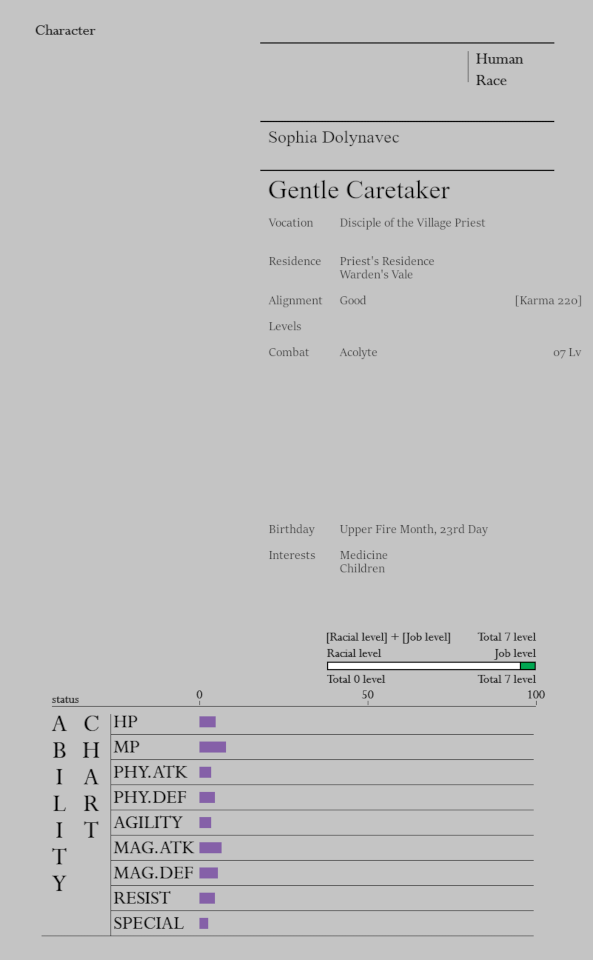
\includegraphics[width=0.8\linewidth]{images/FydzDim.png}
    \caption*{Sophia Dolynavec Character Sheet}
    \label{fig:placeholder}
\end{figure}

\section*{Class Highlight: Acolyte}
As Civilization spreads its light over lands wrested from the wilds and tamed by the hands of its people, powerful institutions rise to serve as pillars of support for their societies. Their many agents, spread throughout the lands, will occasionally discover promising individuals who answer a call beyond that of their everyday lives and these men and women are encouraged to enter their hallowed halls. The most esteemed of orders may even receive regular applicants who petition to become candidates to walk the sacred ways.

 

Just as Paladin Orders induct Squires to join their ranks, the Acolyte is the path of the supplicant who seeks a life of the cloth in civilized realms. From students attending the halls of shining colleges in vast theocracies, to humble disciples aiding the local village priest, Acolytes explore what it is to be an agent of divinity – to be a representative of the gods; whether it is in service to the downtrodden, or in pitched combat against enemies of the faith. This career path may be entirely academic, buried in the practical realities of front line civilian work, or even life-threatening in the case of those who rise through service in tumultuous battlefronts. However, they are generally encouraged to experience the full breadth of what being in service to the faith entails throughout their tenure.

 

Through this sampling of life as a member of the clergy, Acolytes develop an understanding of their personal calling and how it fits within the complicated framework of their theology, working to become increasingly proficient in the paths that answer it. Upon ordainment, the Acolyte will have a well defined vision of their own future, and their levels are converted into the appropriate Cleric-related job classes that lead to its fulfilment.